\documentclass[12pt, fullpage,letterpaper]{article}

\usepackage[margin=1in]{geometry}
\usepackage{url}
\usepackage{amsmath}
\usepackage{amssymb}
\usepackage{xspace}
\usepackage{graphicx}
\usepackage{hyperref}
\usepackage{cancel}
\usepackage{bbm}
%\usepackage{graphicx}
%\usepackage{subfig}
\usepackage{hyperref}
\usepackage{xcolor}
\usepackage{ulem}
\usepackage{cancel}
\usepackage{float}

\newcommand{\beps}{\boldsymbol{\varepsilon}}

\def\red{\color{black!30!red}}
\def\blue{\color{blue}}
\def\blackblue{\color{black!40!blue}}


\newcommand{\semester}{Spring 2022}
\newcommand{\assignmentId}{5}
\newcommand{\releaseDate}{15 Apr, 2022}
\newcommand{\dueDate}{11:59pm, 2 May, 2022}
\newcommand\independent{\protect\mathpalette{\protect\independenT}{\perp}}
\def\independenT#1#2{\mathrel{\rlap{$#1#2$}\mkern2mu{#1#2}}}

\newcommand{\bx}{{\bf x}}
\newcommand{\bw}{{\bf w}}

\title{CS 6190: Probabilistic Machine Learning \semester}
\author{Homework \assignmentId\\ 
{\red Meysam Alishahi (U1323606)}}
\date{Handed out: \releaseDate\\
  Due: \dueDate}

\begin{document}
\maketitle

% Math commands by Thomas Minka
\newcommand{\var}{{\rm var}}
\newcommand{\Tr}{^{\rm T}}
\newcommand{\vtrans}[2]{{#1}^{(#2)}}
\newcommand{\kron}{\otimes}
\newcommand{\schur}[2]{({#1} | {#2})}
\newcommand{\schurdet}[2]{\left| ({#1} | {#2}) \right|}
\newcommand{\had}{\circ}
\newcommand{\diag}{{\rm diag}}
\newcommand{\invdiag}{\diag^{-1}}
\newcommand{\rank}{{\rm rank}}
% careful: ``null'' is already a latex command
\newcommand{\nullsp}{{\rm null}}
\newcommand{\tr}{{\rm tr}}
\renewcommand{\vec}{{\rm vec}}
\newcommand{\vech}{{\rm vech}}
\renewcommand{\det}[1]{\left| #1 \right|}
\newcommand{\pdet}[1]{\left| #1 \right|_{+}}
\newcommand{\pinv}[1]{#1^{+}}
\newcommand{\erf}{{\rm erf}}
\newcommand{\hypergeom}[2]{{}_{#1}F_{#2}}

% boldface characters
\renewcommand{\a}{{\bf a}}
\renewcommand{\b}{{\bf b}}
\renewcommand{\c}{{\bf c}}
\renewcommand{\d}{{\rm d}}  % for derivatives
\newcommand{\e}{{\bf e}}
\newcommand{\f}{{\bf f}}
\newcommand{\g}{{\bf g}}
\newcommand{\h}{{\bf h}}
%\newcommand{\k}{{\bf k}}
% in Latex2e this must be renewcommand
\renewcommand{\k}{{\bf k}}
\newcommand{\m}{{\bf m}}
\newcommand{\mb}{{\bf m}}
\newcommand{\n}{{\bf n}}
\renewcommand{\o}{{\bf o}}
\newcommand{\p}{{\bf p}}
\newcommand{\q}{{\bf q}}
\renewcommand{\r}{{\bf r}}
\newcommand{\s}{{\bf s}}
\renewcommand{\t}{{\bf t}}
\renewcommand{\u}{{\bf u}}
\renewcommand{\v}{{\bf v}}
\newcommand{\w}{{\bf w}}
\newcommand{\x}{{\bf x}}
\newcommand{\y}{{\bf y}}
\newcommand{\z}{{\bf z}}
%s\newcommand{\l}{\boldsymbol{l}}
\newcommand{\A}{{\bf A}}
\newcommand{\B}{{\bf B}}
\newcommand{\C}{{\bf C}}
\newcommand{\D}{{\bf D}}
\newcommand{\E}{{\bf E}}
\newcommand{\F}{{\bf F}}
\newcommand{\G}{{\bf G}}
\renewcommand{\H}{{\bf H}}
\newcommand{\I}{{\bf I}}
\newcommand{\J}{{\bf J}}
\newcommand{\K}{{\bf K}}
\renewcommand{\L}{{\bf L}}
\newcommand{\M}{{\bf M}}
\newcommand{\N}{\mathcal{N}}  % for normal density
\newcommand{\Dcal}{\mathcal{D}}  % for normal density

%\newcommand{\N}{{\bf N}}
\renewcommand{\O}{{\bf O}}
\renewcommand{\P}{{\bf P}}
\newcommand{\Q}{{\bf Q}}
\newcommand{\R}{{\bf R}}
\renewcommand{\S}{{\bf S}}
\newcommand{\T}{{\bf T}}
\newcommand{\U}{{\bf U}}
\newcommand{\V}{{\bf V}}
\newcommand{\W}{{\bf W}}
\newcommand{\X}{{\bf X}}
\newcommand{\Y}{{\bf Y}}
\newcommand{\Z}{{\bf Z}}

% this is for latex 2.09
% unfortunately, the result is slanted - use Latex2e instead
%\newcommand{\bfLambda}{\mbox{\boldmath$\Lambda$}}
% this is for Latex2e
\newcommand{\bfLambda}{\boldsymbol{\Lambda}}

% Yuan Qi's boldsymbol
\newcommand{\bsigma}{\boldsymbol{\sigma}}
\newcommand{\balpha}{\boldsymbol{\alpha}}
\newcommand{\bpsi}{\boldsymbol{\psi}}
\newcommand{\bphi}{\boldsymbol{\phi}}
\newcommand{\boldeta}{\boldsymbol{\eta}}
\newcommand{\Beta}{\boldsymbol{\eta}}
\newcommand{\btau}{\boldsymbol{\tau}}
\newcommand{\bvarphi}{\boldsymbol{\varphi}}
\newcommand{\bzeta}{\boldsymbol{\zeta}}

\newcommand{\blambda}{\boldsymbol{\lambda}}
\newcommand{\bLambda}{\mathbf{\Lambda}}
\newcommand{\bOmega}{\mathbf{\Omega}}
\newcommand{\bomega}{\mathbf{\omega}}
\newcommand{\bPi}{\mathbf{\Pi}}

\newcommand{\btheta}{\boldsymbol{\theta}}
\newcommand{\bpi}{\boldsymbol{\pi}}
\newcommand{\bxi}{\boldsymbol{\xi}}
\newcommand{\bSigma}{\boldsymbol{\Sigma}}

\newcommand{\bgamma}{\boldsymbol{\gamma}}
\newcommand{\bGamma}{\mathbf{\Gamma}}

\newcommand{\bmu}{\boldsymbol{\mu}}
\newcommand{\1}{{\bf 1}}
\newcommand{\0}{{\bf 0}}

% \newcommand{\comment}[1]{}

\newcommand{\bs}{\backslash}
\newcommand{\ben}{\begin{enumerate}}
\newcommand{\een}{\end{enumerate}}

 \newcommand{\notS}{{\backslash S}}
 \newcommand{\nots}{{\backslash s}}
 \newcommand{\noti}{{\backslash i}}
 \newcommand{\notj}{{\backslash j}}
 \newcommand{\nott}{\backslash t}
 \newcommand{\notone}{{\backslash 1}}
 \newcommand{\nottp}{\backslash t+1}
% \newcommand{\notz}{\backslash z}

\newcommand{\notk}{{^{\backslash k}}}
%\newcommand{\noti}{{^{\backslash i}}}
\newcommand{\notij}{{^{\backslash i,j}}}
\newcommand{\notg}{{^{\backslash g}}}
\newcommand{\wnoti}{{_{\w}^{\backslash i}}}
\newcommand{\wnotg}{{_{\w}^{\backslash g}}}
\newcommand{\vnotij}{{_{\v}^{\backslash i,j}}}
\newcommand{\vnotg}{{_{\v}^{\backslash g}}}
\newcommand{\half}{\frac{1}{2}}
\newcommand{\msgb}{m_{t \leftarrow t+1}}
\newcommand{\msgf}{m_{t \rightarrow t+1}}
\newcommand{\msgfp}{m_{t-1 \rightarrow t}}

\newcommand{\proj}[1]{{\rm proj}\negmedspace\left[#1\right]}
\newcommand{\argmin}{\operatornamewithlimits{argmin}}
\newcommand{\argmax}{\operatornamewithlimits{argmax}}

\newcommand{\dif}{\mathrm{d}}
\newcommand{\abs}[1]{\lvert#1\rvert}
\newcommand{\norm}[1]{\lVert#1\rVert}

%miscellaneous symbols
\newcommand{\ie}{{{i.e.,}}\xspace}
\newcommand{\eg}{{{\em e.g.,}}\xspace}
\newcommand{\EE}{\mathbb{E}}
\newcommand{\VV}{\mathbb{V}}
\newcommand{\sbr}[1]{\left[#1\right]}
\newcommand{\rbr}[1]{\left(#1\right)}
\newcommand{\cmt}[1]{}



\footnotesize
	\begin{itemize}
		\item You are welcome to talk to other members of the class about
		the homework. I am more concerned that you understand the
		underlying concepts. However, you should write down your own
		solution. Please keep the class collaboration policy in mind.
		
		\item Feel free discuss the homework with the instructor or the TAs.
		
		\item Your written solutions should be brief and clear. You need to
		show your work, not just the final answer, but you do \emph{not}
		need to write it in gory detail. Your assignment should be {\bf no
			more than 10 pages}. Every extra page will cost a point.
		
		\item Handwritten solutions will not be accepted.
		
		\item The homework is due by \textbf{midnight of the due date}. Please submit
		the homework on Canvas.
	\end{itemize}

%GMM
%Bayes logistic regression, VB, Laplace, Laplace Hession, 
%LDA 

\section*{Practice  [100 points + 70 bonus]}	
\label{sec:q1}
\begin{enumerate}
	\item~[30 points] For warm-up, let us deal with the same scalar distribution in the last homework, 
	\[
	p(z) \propto \exp(-z^2)\sigma(10z + 3).
	\]
	You will implement MCMC algorithms to sample from this distribution. To reach the burn-in stage, please run your chain for $100K$ iterations(\ie generate $100K$ samples). Then continue to run $50K$ iterations, pick every $10$-th sample to obtain your final samples.  Set your initial sample to $0$.
	\begin{enumerate}
		\item~[14 points] Implement Metroplis-Hasting, with Gaussian proposal, $q(z_{n+1}|z_n) = \N(z_{n+1}|z_{n}, \tau)$. Vary $\tau$ from $\{0.01, 0.1, 0.2, 0.5, 1\}$. Run your chain. For each setting of $\tau$, record the acceptance rate (\ie how many candidate samples are accepted/the total number of candidate samples generated). Draw a figure, where the x-axis represents the setting of $\tau$, and y-axis the acceptance rate. What do you observe?
		For each setting of $\tau$, draw a figure, show a normalized hist-gram of the $5K$ samples you collected. Please set the number of bins to $50$. If you use Python, please use matplotlib and look up the API at \url{https://matplotlib.org/3.1.1/api/_as_gen/matplotlib.pyplot.hist.html}. You can set the parameter ``bins'' to 50 and ``density'' to true. Also, please draw the ground-truth density curve (obtained via quadrature --- you did that in the last homework). Now what do you observe?\\
{\bf \red Answer: }{\blackblue 
See  Figure \ref{Fig2}. 
	\begin{figure}[H]
	\begin{center}
     	\frame{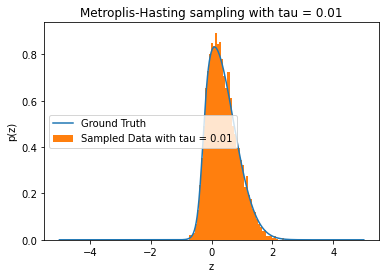
\includegraphics[width=0.3 \linewidth]{Images/Q1/a/MHtau1.png}}
     	\frame{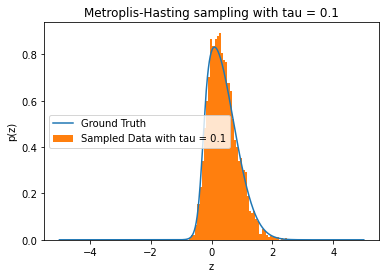
\includegraphics[width=0.3 \linewidth]{Images/Q1/a/MHtau2.png}}
     	\frame{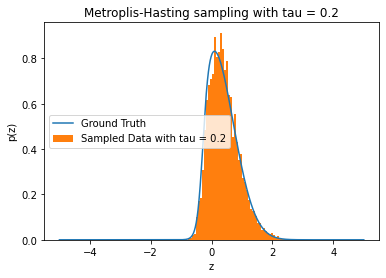
\includegraphics[width=0.3 \linewidth]{Images/Q1/a/MHtau3.png}}
     	\frame{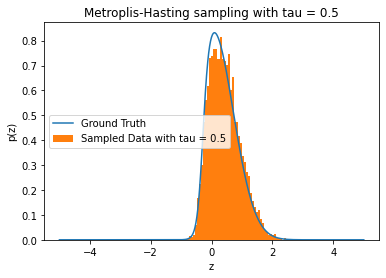
\includegraphics[width=0.3 \linewidth]{Images/Q1/a/MHtau4.png}}
     	\frame{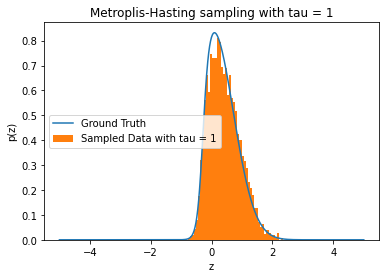
\includegraphics[width=0.3 \linewidth]{Images/Q1/a/MHtau5.png}}
     	\frame{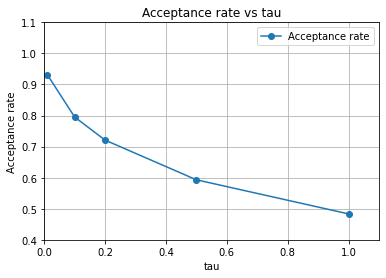
\includegraphics[width=0.3 \linewidth]{Images/Q1/a/AccVsTau.png}}
	 \end{center}
	 \caption{{\footnotesize Metroplis-Hasting with Gaussian proposal and  $\tau$ from $\{0.01, 0.1, 0.2, 0.5, 1\}$}}\label{Fig2}    
	\end{figure}	
}		
		\item~[14 points] Implement Hybrid Monte-Carlo sampling with Leapfrog. Let us fix $L = 10$, and vary $\epsilon$ from $\{0.005, 0.01, 0.1, 0.2, 0.5\}$. Run your chain. Similar to the above, for each setting of $\epsilon$, record the acceptance rate,and draw a figure showing $\epsilon$ \textit{v.s.} acceptance rate. What do you observe? For each setting of $\epsilon$, draw the normalized hist-gram ($50$ bins)of collected $5K$ samples. what do you observe? You can leverage the third-party implementation of leap-frog algorithm if you feel it is too difficult to implement it by yourself. One example is given by \url{https://people.sc.fsu.edu/~jburkardt/py_src/leapfrog/leapfrog.py}. However, using the third-party implementation of HMC (\eg hamiltorch) is NOT allowed. We expect you do understand and are able to implement the algorithmic steps of HMC. \\
{\bf \red Answer: }{\blackblue 
See  Figure \ref{Fig1}. 
	\begin{figure}[H]
	\begin{center}
     	\frame{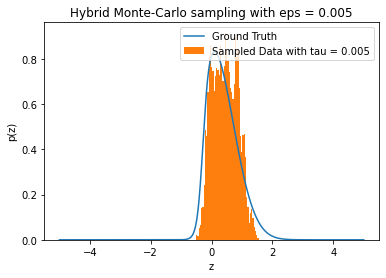
\includegraphics[width=0.3 \linewidth]{Images/Q1/b/HMCeps1.png}}
     	\frame{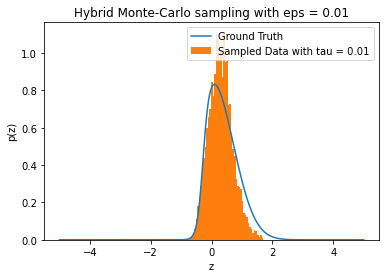
\includegraphics[width=0.3 \linewidth]{Images/Q1/b/HMCeps2.png}}
     	\frame{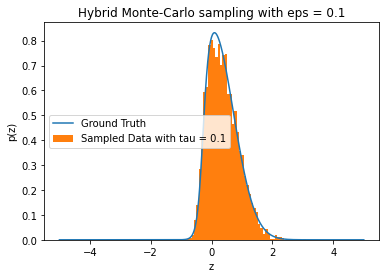
\includegraphics[width=0.3 \linewidth]{Images/Q1/b/HMCeps3.png}}
     	\frame{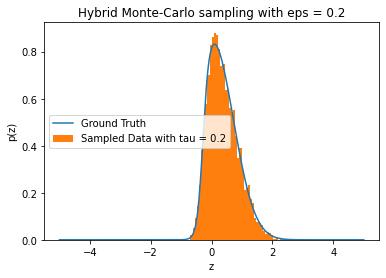
\includegraphics[width=0.3 \linewidth]{Images/Q1/b/HMCeps4.png}}
     	\frame{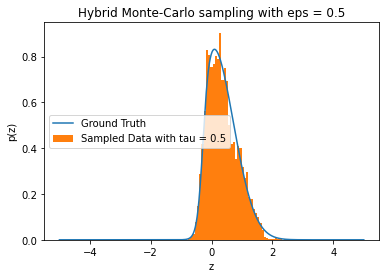
\includegraphics[width=0.3 \linewidth]{Images/Q1/b/HMCeps5.png}}
     	\frame{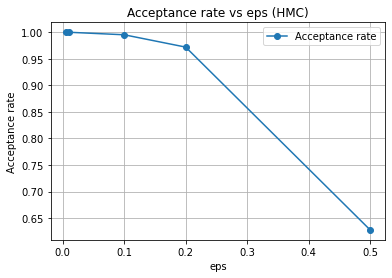
\includegraphics[width=0.3 \linewidth]{Images/Q1/b/AccVsEps.png}}
	 \end{center}
	 \caption{{\footnotesize Hybrid Monte-Carlo sampling with Leapfrog ($L=10$) and  $\epsilon$ from $\{0.005, 0.01, 0.1, 0.2, 0.5\}$}}\label{Fig1}    
	\end{figure}	
}
		
		\item~[2 points] Now compare the results from the two MCMC algorithms, what do you observe and conclude? \\
{\bf \red Answer: }{\blackblue 
Comparing the acceptance rates, we can see that the Hybrid Monte-Carlo sampling is working much better, especially for small values of $\epsilon$.  
The reason is that the Hybrid Monte-Carlo sampling uses gradient base information to explore distribution more effectively.  
}
	\end{enumerate}

	\item~[20 points] Let us work with a 2-dimensional Gaussian distribution, 
	\[
	p(z_1, z_2) = \N(\left[\begin{array}{c}z_1\\z_2
	\end{array}\right] | \left[\begin{array}{c}0\\0
	\end{array}\right], \left[\begin{array}{cc} 3 & 2.9\\2.9 & 3\end{array} \right])
	\]
	\begin{enumerate}
		\item~[2 point] Draw $500$ samples from this distribution and show the scatter plot. What do you observe?\\
{\bf \red Answer: }{\blackblue 
See the left image in Figure \ref{Fig3}. It is observable that the mass of the distribution is concentrated along the line $z_1=z_2$ and near the origin. 
It means that $z_1$ and $z_2$ are highly correlated. 
}
		\item~[10 points] Implement Gibbs sampling to alternatively sample $z_1$ and $z_2$. Set your initial sample to $(-4, -4)$. Run your Gibbs sampler for $100$ iterations. Draw the trajectory of the samples. What do you observe?\\
		{\bf \red Answer: }{\blackblue 
For the plot, see the middle image in Figure \ref{Fig3}. 
The result of Gibbs sampling is satisfying however some parts of the distribution are not explored which is due to the high correlation between consecutive samples in Gibbs sampling method. 
}
		\item~[8 points] Implement HMC with Leapfrog, set $\epsilon = 0.1$ and $L=20$. Run your HMC for $100$ iterations. Set your initial sample to $(-4, -4)$. Draw the trajectory of the samples. What do you observe? Compare with the results of Gibbs sampling, what do you conclude?\\
		{\bf \red Answer: }{\blackblue 
For the plot, see the right image in Figure \ref{Fig3}. 
Compared to Gibbs sampling, it seems that HMC could explore the entire distribution in a more effective way. 
}
		
\begin{figure}[H]
	\begin{center}
     	\frame{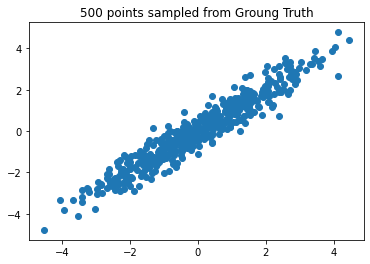
\includegraphics[width=0.3 \linewidth]{Images/Q2/a.png}}
     	\frame{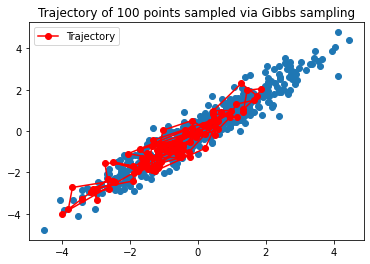
\includegraphics[width=0.3 \linewidth]{Images/Q2/b.png}}
     	\frame{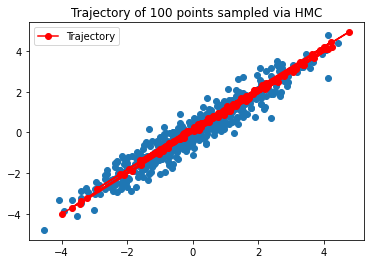
\includegraphics[width=0.3 \linewidth]{Images/Q2/c.png}}
	 \end{center}
	 \caption{{\footnotesize Gibbs sampling vs HMC with Leapfrog ($L=20$)}}\label{Fig3}    
	\end{figure}
	\end{enumerate}

	\item~[70 points] Let us work on a real-world dataset we have met before. Please download the data from the folder``data/bank-note''. The features and labels are listed in the file ``data-desc.txt''. The training data are stored in the file ``train.csv'', consisting of $872$ examples. The test data are stored in ``test.csv'', and comprise of $500$ examples. In both the training and testing datasets, feature values and labels are separated by commas. 
	 
	\begin{enumerate}
		\item~[20 points] We assign the feature weight vector $\w$ a standard normal prior $\N(\0, \I)$. Write down the joint probability of the Bayesian logistic regression model. Now, implement HMC with Leapfrog. Set your initial sample to be $\0$. Run your chain for $100K$ iterations to reach the burn-in state; then continue to run $10K$ iterations, pick every $10$-th sample to obtain your posterior samples. Vary $\epsilon$ from $\{0.005, 0.01, 0.02, 0.05\}$ and $L$ from $\{10, 20, 50\}$. As we did before, we can test the predictive accuracy and predictive log-likelihood. Both can involve the posterior distribution of the weights. How? To evaluate the accuracy, for each posterior sample of $\w$ in hand ($1K$ in total), we can use it to make the predictions ($1$ or $0$) on all the test examples and calculate the accuracy. Then we average the prediction accuracy of all the posterior samples of $\w$. In the same way, we can compute the predictive likelihood. Now you can sense how convenient with posterior samples ---  the integration over posterior distribution is turned to the average across posterior samples! List a table showing different combinations of $\epsilon$ and $\L$ and the resulting predictive accuracy, predictive log-likelihood, and acceptance rate.  What do you observe and conclude?\\
{\bf \red Answer: }{\blackblue 
We know that 
\begin{align*}
p(\mathcal{D}, \w) & = p(\w)p(\mathcal{D}|\w)\\
& = \N(\w|\0,\I)\prod_{i=1}^Np(\t_i|\x_i,\w)\\
& = \N(\w|\0,\I)\prod_{i=1}^Np(\t_i|\x_i,\w)\\
& = \N(\w|\0,\I)\prod_{i=1}^N\left[\sigma(\w^\top\x_i)^{t_i}(1-\sigma(\w^\top\x_i))^{1-t_i}\right]
\end{align*}
and therefore, 
$$U(\w) = \frac{1}{2}\w^\top \w - \sum_{i=1}^N \left[t_i\log\sigma(\w^\top\x_i) + (1-t_i)\log(1-\sigma(\w^\top\x_i))\right] + C$$
and 
\begin{align*}
dU & = \w - \sum_{i=1}^N \Big[t_i(1-\sigma(\w^\top\x_i)) - (1-t_i)\sigma(\w^\top\x_i) \Big]\x_i\\
& = \w + \sum_{i=1}^N \Big[\sigma(\w^\top\x_i) - t_i\Big]\x_i.
\end{align*}
We also set $K(\r) = \frac{1}{2}\r^\top \M^{-1}\r$ and $H(\r,\w) = U(\w) + K(\r)$ where $\M$ is here identity matrix. 
\begin{center}
\begin{tabular}{ |c||c|c|c|c|c|}
 \hline
 \multicolumn{5}{|c|}{Posterior in Bayesian logistic regression model via HMC with Leapfrog} \\
 \hline
 $\epsilon$& $L$ & Predictive accuracy & Predictive log-likelihood & Acceptance rate\\
 \hline
 $0.005$   & $10$    & $98.87\%$ &   $-0.0310$ & $0.9985$\\
 \hline
 $0.005$   & $20$    & $98.87\%$ &   $-0.0299$ & $0.9993$\\
 \hline
 $0.005$   & $50$    & $99.05\%$ &  $-0.0317$  & $0.9989$\\
  \hline
  \hline
 $0.01$   & $10$    & $98.82\%$ &   $-0.0284$ & $0.9964$\\  
 \hline
 $0.01$   & $20$    & $98.95\%$ &   $-0.0337$ & $0.9960$\\
\hline
 $0.01$   & $50$    & $98.89\%$ &   $-0.0296$ & $0.9951$\\
 \hline
 \hline
 $0.02$   & $10$    & $98.76\%$ &   $-0.0334$ & $0.9841$\\  
 \hline
 $0.02$   & $20$    & $98.84\%$ &   $-0.0309$ & $0.9789$\\
\hline
 $0.02$   & $50$    &98.75\%&   $-0.0303$ & $0.9805$\\ 
 \hline
 \hline
 $0.05$   & $10$    & $44.20\%$ &  $ -0.6931$   & $0.0^*$\\  
 \hline
 $0.05$   & $20$    & $44.20\%$ &    $-0.6931$  & $0.0$\\
\hline
 $0.05$   & $50$    & $44.20\%$ &    $-0.6931$  & $0.0$\\
 \hline
\end{tabular}
\end{center}
{\red * For the last three rows (for $\epsilon = 0.05$ and $L=10,20,50$), no sample has been accepted, and the only sample by which the accuracy and log-likelihood are computed based on it is the initial point $\0$. }


One can see that HMC is doing its job pretty well when $\epsilon$ is small even if $L$ is large. 
However, for $\epsilon = 0.05$, we can see that the acceptance rate become $0$ which results in no sampling at all.  This is indeed reasonable because using a big step as $\epsilon = 0.05$ and Leapfrog many times results in a large numerical error. 
}
		
		\item~[20 points][\textbf{Bonus}]. We will implement Gibbs sampling for linear classification. However, Bayesian logistic regression does not allow tractable conditional posteriors. So we will use the Bayesian probit model with augmented variables. We have discussed it before in our class, if you cannot remember, please check our slides regarding generalized linear models. Again, we will assign a standard normal prior over $\w$. For each training sample $n$, we introduce an auxiliary variable $z_n$. The joint probability is given by
		\begin{align}
		p(\w, \z, \Dcal) = \N(\w|\0, \I)\prod_n \N(z_n|\w^\top \x_n, 1)\mathbbm{1}\big((2y_n-1)z_n\ge 0\big) \label{eq:aug}
		\end{align}
		where $\z = [z_1, z_2, \ldots, z_N]^\top$, and $\mathbbm{1}(\cdot)$ is the indicator function. Note that if we marginalize out $\z$, we will recover the original Probit model, 
		\begin{align}
		&p(\w, \z, \Dcal) = \N(\w|\0, \I)\prod_n \phi\big((2y_n-1)\w^\top \x_n\big) \notag \\
		&=\N(\w|\0, \I)\prod_n \mathrm{Bern}\big(y_n|\phi(\w^\top \x_n)\big), \label{eq:probit}
		\end{align}
		where $\phi(\cdot)$ is the CDF of the standard normal distribution, $\phi(x) = \int_\infty^x \N(t|0, 1)\d t$. Note that Bayesian logistic regression just replaces $\phi(\cdot)$ by the Sigmoid activation function. Now implement your Gibbs sampling algorithm based on the augmented version \eqref{eq:aug}. Alternatively sample $\w$ and each $z_n$. Note that the conditional posterior of each $z_n$ will be a truncated Gaussian. You can use \texttt{scipy.stats.truncnorm} to generate samples (or implement by yourself). Before coding, please list your derivation of the conditional posteriors. Run your chain for $100K$ iterations to reach the burn-in stage; then continue to run $10K$ iterations, pick every $10$-th sample to obtain your final posterior samples. Now compute and report the predictive accuracy and log-likelihood with your posterior samples. Note that your predictive log-likelihood should be based on the original model \eqref{eq:probit}, rather than the augmented one. How does the performance compare with HMC on Bayesian logistic regression model?\\
{\bf \red Answer: }{\blackblue 
Set $\X$ to be an $N \times d$ whose rows are corresponding to data pointsn $\x_n$'s.
If $\z \sim p(\z| \w, \Dcal)$, then 
\begin{align*}
\log p(\w| \z, \Dcal) & = \log\N(\w|\0, \I)\prod_n \N(z_n|\w^\top \x_n, 1)\underbrace{\mathbbm{1}\big((2y_n-1)z_n\ge 0\big)}_{ = 1} + C\\
& = - \frac{1}{2}\w^\top \left[\mathbf{I}_d - \sum\limits_{n=1}^N \x_n\x_n^\top\right]\w + \w^\top\sum\limits_{n = 1}^N z_n  \x_n + C\\
& = - \frac{1}{2}\w^\top \left[ \mathbf{I}_d - \X^\top \X \right]\w + \w^\top \sum\limits_{n = 1}^N z_n  \x_n + C\\
& = - \frac{1}{2}\w^\top \left[ \mathbf{I}_d - \X^\top \X \right]\w +  \z^\top  \X \w + C.
\end{align*}
This concludes 
$$\w| \z, \Dcal \sim \N(\bmu, \bSigma)\quad\quad \quad \text{ where } \quad\quad \quad \bSigma^{-1} = \mathbf{I}_d - \X^\top \X,\  \bmu = \bSigma\X^\top\z.
$$
Also, when $\w$ is given it is clear that for each $n$
\begin{align*}
z_n |\w,\Dcal\quad & \propto \quad \N(z_n|\w^\top \x_n, 1)\mathbbm{1}\big((2y_n-1)z_n\ge 0\big)\\ \\
& = \left\{\begin{array}{cc}
\mathcal{TN}(\mu =\w^\top \x_n , \sigma =1 , a =-\infty , b = 0 ) & \quad \text{if} \quad y_n = 0\\ \\
\mathcal{TN}(\mu =\w^\top \x_n , \sigma =1 , a =0 , b =\infty  ) &  \quad \text{if} \quad y_n = 1,\\
\end{array}\right.
\end{align*}
where $\mathcal{TN}(\mu,\sigma, a, b)$ stands for  truncated normal distribution with mean $\mu$ and variance $\sigma^2$ in interval $[a,b]$.

Using Gibbs sampling, we obtain:\\
{\bf Predictive accuracy: } $98.8$ \\
{\bf Predictive log-likelihood: } $-0.02897856072681373$\\
It seems that both models (Gibbs sampling for Bayesian probit model with augmented variables and HMC on Bayesian logistic regression) work pretty well. 
}
		
\item~[28 points] Finally, we will implement a Bayesian neural network (NN). We will use two intermediate layers, and each layer has the same number of nodes. Vary the number of nodes from $[10, 20, 50]$. Vary the activation function from \{\texttt{tanh}, \texttt{RELU}\}. 	We will use a factorized Gaussian posterior for the NN weights (check out the slides). We will assign a standard normal prior over each weight. The output of the NN will be thrown into a Sigmoid activation function, with which we obtain a Bernoulli likelihood. Please use PyTorch or TensorFlow to implement the \texttt{Bayes by BP} algorithm based on the reparameterization trick plus stochastic optimization. If you prefer other automatic differential library (\eg JAX) , that is totally OK. But please do NOT  implement BP by yourself --- it is a waste of time. Note that you do not need to sample mini-batches in this problem --- because the training set is small. Please use Adam algorithm for stochastic optimization. You can tune the base learning rate from \{1e-3, 0.5e-3, 1e-4, 1e-5\} to find the best result for each layer-width and activation function setting. Initialize posterior mean and variance of each weight to be $0$ and $1$, respectively. Run the Adam algorithm for 1,000 iterations. For each layer width and activation function setting, calculate the predictive log-likelihood and accuracy. How? Use Monte-Carlo approximation. Check out the slides.  Use the variational posterior to generate $100$ samples for the weight vector; With each sample, you can calculate the prediction accuracy and log-likelihood on the test dataset; finally, you report the average results.  To check the behaviour of your BNN, let us pick up one setting: the number of node is 20 and the activation function is \texttt{tanh}. For each iteration,  please use the current posterior mean of the weights to compute the average log-likelihood on the training set and test set respectively. Draw two plots, one plot showing how the training log-likelihood varies along with the number of iterations, the other showing how the test log-likelihood varies along with the number of iterations. What do you observe and conclude?\\
{\bf \red Answer: }{\blackblue 
Let'e remind that $P(\mathcal{W}) = \prod\limits_{w\in\mathcal{W}}\N(w|0,1)$. Also, 
we have the assumption that the posterior is fully fatctorized Gaussian, i.e, 
\begin{align*}
q(\mathcal{W}) &  = \prod_i q(w_i) = \prod_i \N\big(w_i|\mu_i, \log(1+\exp(\rho_i))\big).
\end{align*}
Our goal is to estimate the paremete $\btheta =\{(\mu_i, \rho_i)\}_i$. We saw in the class that 
\begin{align*}
\log(p(\mathcal{D})) & \geq \mathcal{L}(\btheta) = \int q(\mathcal{W})\log\frac{p(\mathcal{W})p(\mathcal{D}|\mathcal{W})}{q(\mathcal{W})}\d\mathcal{W}\\
& = \sum_i \mathbb{E}_{q(w_i)}\big[\log p(w_i)\big] + \sum_{n=1}^N \mathbb{E}_{q(\mathcal{W})} \big[\log p(y_n | f_{\mathcal{W}}(\x_n)\big] 
+ \sum_i H(q(w_i))\\
& = \sum_i \mathbb{E}_{q(w_i)}\big[\log p(w_i)\big] + \mathbb{E}_{p(\beps)} \big[\log p(y_n | f_{\mathcal{W}}(\x_n)\big] 
+ \sum_i H(q(w_i))
\end{align*}
where $\mathcal{W} = T(\btheta,\beps)$ and $\beps\sim \N(\mathbf{0}, \mathbf{I})$ (indeed, $w_i = \mu_i+\varepsilon \sqrt{\log(1+\exp(\rho_i))}$).
Note that 
\begin{align*}
\mathbb{E}_{q(w_i)}\big[\log p(w_i)\big] & = -\frac{1}{2}\mathbb{E}_{q(w_i)}\big[w_i^2\big] + C\\
& = -\frac{1}{2}\left(\var(w_i) + \mathbb{E}(w_i^2)\right)+ C\\
& =  -\frac{1}{2}\left(\log(1+\exp(\rho_i)) + \mu_i^2\right)  + C
\end{align*}
 and 
 \begin{align*}
H\left(q(w_i)\right) & = \frac{1}{2\sigma_i^2}\mathbb{E}_{q(w_i)}\big[(w_i -\mu_i)^2\big] + \log(\sigma_i) + C\\
& = \frac{1}{2}\log(\log(1+\exp(\rho_i))) + C.
\end{align*}
This implies that 
$$\mathcal{L}(\btheta) = \frac{1}{2}\sum_i\Big(-\mu_i^2 - \log(1+\exp(\rho_i)) +  \log(\log(1+\exp(\rho_i)))\Big) + \mathbb{E}_{p(\beps)} \big[\log p(y_n | f_{\mathcal{W}}(\x_n)\big] .$$


\begin{center}
\begin{tabular}{ |c||c|c|c|c|c|}
 \hline
 \multicolumn{5}{|c|}{Performance of Bayesian linear classification with \texttt{ReLU} acctivation} \\
 \hline
Learning rate & Hidden layer size & Test accuracy & Train log-likelihood &  Test log-likelihood\\
 \hline
 1e-3   & $10$    & $99.66\%$ &   $-0.0101$ & $-0.0126$\\ 
 \hline
 1e-3   & $20$    & $99.59\%$ &   $-0.0109$ & $-0.0124$\\
 \hline
 1e-3   & $50$    & $99.68\%$ &  $-0.0097$  & $-0.0107$\\
  \hline
  \hline
 0.5e-3   & $10$    & $99.20\%$ &   $-0.0262$ & $-0.0296$\\  
 \hline
 0.5e-3   & $20$    & $99.42\%$ &   $-0.0175$ & $-0.0199$\\
\hline
 0.5e-3   & $50$    & $99.61\%$ &   $-0.0119$ & $-0.0142$\\
 \hline
 \hline
 1e-4   & $10$    & $57.77\%$ &   $-0.5895$ & $-0.5902$\\  
 \hline
 1e-4   & $20$    & $78.97\%$ &   $-0.4813$ & $-0.4781$\\
\hline
 1e-4   & $50$    & $95.92\%$ &   $-0.1675$ & $-0.1646$ \\ 
 \hline
 \hline
 1e-5   & $10$    & $52.94\%$ & $-0.6909$     &  $-0.6911$\\  
 \hline
 1e-5   & $20$    & $53.40\%$ &   $-0.6913$ & $-0.6910$\\
\hline
 1e-5   & $50$    & $58.56\%$ &   $-0.6775$  & $-0.6786$\\
 \hline
\end{tabular}
\end{center}
We can see that the Bayesian NN with \texttt{ReLU} acctivation function is working nice for learning rates $1e-3, 0.5e-3$ and for each layer size $10,20,30$. However, the best performance is recorded in $lr =1e-3$ and $size = 50$.


\begin{center}
\begin{tabular}{ |c||c|c|c|c|c|}
 \hline
 \multicolumn{5}{|c|}{Performance of Bayesian linear classification with \texttt{Tanh} acctivation} \\
 \hline
Learning rate & Hidden layer size & Test accuracy & Train log-likelihood &  Test log-likelihood\\
 \hline
 1e-3   & $10$    & $98.67\%$ &   $-0.0385$ & $-0.0391$\\ 
 \hline
 1e-3   & $20$    & $99.07\%$ &   $-0.0251$ & $-0.0264$\\
 \hline
 1e-3   & $50$    & $99.20\%$ &  $-0.0211$  & $-0.0229$\\
  \hline
  \hline
 0.5e-3   & $10$    & $98.58\%$ &   $-0.0534$ & $-0.0550$\\  
 \hline
 0.5e-3   & $20$    & $98.60\%$ &   $-0.0391$ & $-0.0409$\\
\hline
 0.5e-3   & $50$    & $98.95\%$ &   $-0.0289$ & $-0.0293$\\
 \hline
 \hline
 1e-4   & $10$    & $86.89\%$ &   $-0.5407$ & $-0.5361$\\  
 \hline
 1e-4   & $20$    & $95.92\%$ &   $-0.3221$ & $-0.3205$\\
\hline
 1e-4   & $50$    & $97.90\%$ &   $-0.1094$ & $-0.1139$ \\ 
 \hline
 \hline
 1e-5   & $10$    & $54.12\%$ & $-0.6908$     &  $-0.6905$\\  
 \hline
 1e-5   & $20$    & $53.45\%$ &   $-0.6897$ & $-0.6900$\\
\hline
 1e-5   & $50$    & $68.04\%$ &   $-0.6547$  & $-0.6536$\\
 \hline
\end{tabular}
\end{center}
In view of the above table, we can see that the Bayesian NN with \texttt{Tanh} acctivation function is working good for learning rates $1e-3, 0.5e-3$ and for each layer size $10,20,30$. However, the best performance is recorded in $lr =1e-3$ and $size = 50$.

Overall, we can conclude that although Bayesian NN  is a strong model, it needs very carefully tunning for its hyperparameters including the choices of activation function, hidden layer architecture, and the learning rate. 
	\begin{figure}[H]
	\begin{center}
     	\frame{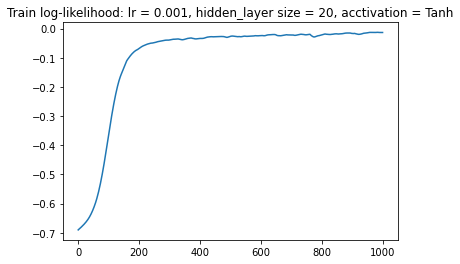
\includegraphics[width=0.45 \linewidth]{Images/Q3/c/trainll.png}}
     	\frame{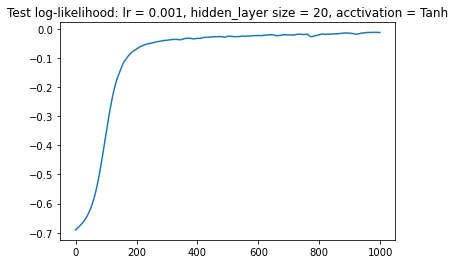
\includegraphics[width=0.45 \linewidth]{Images/Q3/c/testll.png}}
	 \end{center}
	 \caption{{\footnotesize Behaviour of BNN with $20$ nodes and \texttt{tanh} as the activation function}}\label{Fig1}    
	\end{figure}	

}
		
		\item~[2 points] Compare the results from Bayesian linear classification and NN models. What do you observe and conclude?\\
{\bf \red Answer: }{\blackblue 
Setting the parameters appropriately, the Bayesian neural network surpasses the Bayesian linear classification a bit. 

}
		
		
		
	\end{enumerate}


	\item~[50 points][\textbf{Bonus}] If you feel addictive to neural networks, this is a good chance to do more state-of-the-art work.
	Please come to the website \url{http://yann.lecun.com/exdb/mnist/} and download the MNIST dataset provided by LeCun et. al. It is a famous benchmark dataset. Your goal is to classify hand-written digits. The dataset includes 60,000 training and 10,000 testing pixel images of size $28 \times 28$. Each image is labelled with its ground-truth number (0-9 inclusive). Please preprocess the data by dividing each pixel values by 126. You will implement two versions of Bayesian neural networks. To select the hyper-parameters, please from the training data randomly select 50,000 digits for training and use the remaining 10,000 digits for validation. After the best hyper-parameters are identified, you train on the whole 60,000 digits again. Your NN output will be $10$ dimensional, which are used to construct the categorical likelihood (\ie softmax) --- check out the slides if you are unclear. Please use Adam for stochastic optimization. We consider to tune the (base) learning rate from \{1e-3, 1e-4, 1e-5\}. 
	We will use two hidden layers, and each layer has the same number of nodes. 
	%$\mathbbm{1}$
	\begin{enumerate}
		\item~[15 points] First, we consider to place an independent standard normal prior over each weight. We use factorized Gaussian posterior (check the slides).  Implement your Bayes by BP algorithm. Please run your algorithm for 1,000 epochs and report the predictive accuracy. The way to compute the predictive accuracy is the same as in Problem 3. Use your variational posterior of the weights to sample $10$ sets of weights, each weight set are used to predict the labels of the test samples (you choose the label with the largest probability in your model as the prediction) and calculate the accuracy; finally you average the $10$ accuracy values. Vary the number of nodes in each hidden layer from \{400, 800, 1200\}. Try both the \texttt{tanh} and \texttt{RELU} activation functions. Report the prediction accuracy for each combination.  \\
{\bf \red Answer: }{\blackblue 
{\bf\red Due to time concerns, we have only run the neural network for $20$ epochs. }		
		\begin{center}
\begin{tabular}{ |c||c|c|c|c|}
 \hline
 \multicolumn{4}{|c|}{Validation accuracy of Bayesian linear classification on MNIST} \\
 \hline
Learning rate & Hidden layer &  Accuracy (\texttt{ReLU}) & Accuracy (\texttt{Tanh})\\
 \hline
 1e-3   & $400$     & $94.85\%$ &   91.27\%\\ 
 \hline
 1e-3   & $800$     & $94.14\%$  &  90.99\%\\
 \hline
 1e-3   & $1200$   & $94.93\%$  &  89.89\%\\
  \hline
 \hline
 1e-4   & $400$      & $88.34\%$&  89.35\%\\  
 \hline
 1e-4   & $800$      & $87.71\%$ &  89.50\%\\
\hline
 1e-4   & $1200$    & $87.28\%$ &  88.39\%\\ 
 \hline
 \hline
 1e-5   & $400$    & $25.56\%$ &  6053\%\\  
 \hline
 1e-5   & $800$    & $32.90\%$ &  59.35\%\\
\hline
 1e-5   & $1200$    & $45.15\%$ &  61.79\%\\
 \hline
\end{tabular}
\end{center}
		
		

}		
		\item~[20 points] Then we consider to assign a spike and slab prior over each weight,
		\[
		p(w_i) = \pi \N(w_i|0, \sigma_1^2) + (1-\pi)\N(w_i|0, \sigma_2^2)
		\]
		where we tune $-\log(\sigma_1) \in \{0, 1, 2\}$ and $-\log(\sigma_2) \in \{6,7,8\}, \pi \in \{\frac{1}{4}, \frac{1}{2}, \frac{3}{4}\}$. We still use the factorized Gaussian posterior. Implement your Bayes by BP algorithm. Run your algorithm for 1,000 epochs. Report the predictive accuracy when the number of nodes in each hidden layer is in \{400, 800, 1200\}, and the activation function is \texttt{tanh} or \texttt{RELU}. Do you observe many weights have very small posterior variances and means close to $0$? Why did this happen?\\
{\bf \red Answer: }{\blackblue 
Similar to  Question~ 3 Part (c),  
\begin{align*}
\log(p(\mathcal{D})) & \geq \mathcal{L}(\btheta)\\
& = \sum_i \mathbb{E}_{q(w_i)}\big[\log p(w_i)\big] + \mathbb{E}_{p(\beps)} \big[\log p(y_n | f_{\mathcal{W}}(\x_n)\big] 
+ \sum_i H(q(w_i))
\end{align*}
where $\mathcal{W} = T(\btheta,\beps)$ and $\beps\sim \N(\mathbf{0}, \mathbf{I})$ (indeed, $w_i = \mu_i+\varepsilon \sqrt{\log(1+\exp(\rho_i))}$).
Again, we have 
 \begin{align*}
H\left(q(w_i)\right) & = \frac{1}{2\sigma_i^2}\mathbb{E}_{q(w_i)}\big[(w_i -\mu_i)^2\big] + \log(\sigma_i) + C\\
& = \frac{1}{2}\log(\log(1+\exp(\rho_i))) + C.
\end{align*}
But now, the term $\mathbb{E}_{q(w_i)}\big[\log p(w_i)\big]$ is untractable. However, with the reparameterization trick, we can rewrite  
$\mathcal{L}(\btheta)$ as follwos:
\begin{align*}
\mathcal{L}(\btheta)
& = \sum_i \mathbb{E}_{p(\epsilon_i)}\big[\log p(w_i)\big] + \mathbb{E}_{p(\beps)} \big[\log p(y_n | f_{\mathcal{W}}(\x_n)\big] 
+ \frac{1}{2}\sum_i  \log(\log(1+\exp(\rho_i)))
\end{align*}
Now, using stochastic optimization, we can maximize $\mathcal{L}(\btheta)$. 


		\begin{center}
\begin{tabular}{ |c||c|c|c|c|}
 \hline
 \multicolumn{4}{|c|}{Validation accuracy of spike and slab prior (BNN) $\pi = 1/4$} \\
 \hline
Learning rate & Hidden layer &  Accuracy (\texttt{ReLU}) & Accuracy (\texttt{Tanh})\\
 \hline
 1e-3   & $400$     & $95.76\%$ &   93.59\%\\ 
 \hline
 1e-3   & $800$     & $94.30\%$  &  91.84\%\\
 \hline
 1e-3   & $1200$   & $94.56\%$  &  91.69\%\\
  \hline
 \hline
 1e-4   & $400$      & $90.18\%$& 87.77\%\\  
 \hline
 1e-4   & $800$      & $90.28\%$ &  90.19\%\\
\hline
 1e-4   & $1200$    & $90.17\%$ &  89.33\%\\ 
 \hline
 \hline
 1e-5   & $400$    & $43.15\%$ &  62.85\%\\  
 \hline
 1e-5   & $800$    & $58.60\%$ &  75.40\%\\
\hline
 1e-5   & $1200$    & $67.39\%$ &  7334\%\\
 \hline
\end{tabular}
\end{center}		
}		

		
		\item~[10 points] Implement the vanilla NN training with SGD --- namely, we only perform MAP estimation. Run 1,000 epochs. Report the prediction accuracy for the same settings as above. Are your results consistent with Table 1 in the paper~\url{https://arxiv.org/pdf/1505.05424.pdf}? Compared with the two version of BNNs, what do you observe and conclude? \\
{\bf \red Answer: }{\blackblue 
		
		
		\begin{center}
\begin{tabular}{ |c||c|c|c|c|}
 \hline
 \multicolumn{4}{|c|}{Validation accuracy of Vanilla NN (SGD) on MNIST} \\
 \hline
Learning rate & Hidden layer &  Accuracy (\texttt{ReLU}) & Accuracy (\texttt{Tanh})\\
 \hline
 1e-3   & $400$     & $91.05\%$ &   91.38\%\\ 
 \hline
 1e-3   & $800$     & $92.59\%$  &  91.61\%\\
 \hline
 1e-3   & $1200$   & $93.41\%$  &  91.79\%\\
  \hline
 \hline
 1e-4   & $400$      & $72.89\%$& 78.83\%\\  
 \hline
 1e-4   & $800$      & $83.34\%$ &  86.67\%\\
\hline
 1e-4   & $1200$    & $86.74\%$ &  88.92\%\\ 
 \hline
 \hline
 1e-5   & $400$    & $12.97\%$ &  17.57\%\\  
 \hline
 1e-5   & $800$    & $26.36\%$ &  47.32\%\\
\hline
 1e-5   & $1200$    & $45.20\%$ &  55.22\%\\
 \hline
\end{tabular}
\end{center}		
}					
		
		
		
		\item~[5 points] Fix the number of nodes per layer to 1,200 and use \texttt{RELU} activation function. For each algorithm, use the validation dataset to choose the best hyper-parameters (e.g., learning rate). With the best hyper-parameter(s), re-run your algorithms on the whole training set, and draw the learning curve --- how does the test accuracy vary along with the number of epochs. Is it consistent with Fig. 2 in the paper~\url{https://arxiv.org/pdf/1505.05424.pdf}? What do you conclude and observe?\\
{\bf \red Answer: }{\blackblue 
		Due to time-consuming, we only run the algorithms for 100 iterations, see~\ref{Fig10}. It is not exactly what is in the paper but it seems that we could see the same behaviours.
			\begin{figure}[H]
	\begin{center}
     	\frame{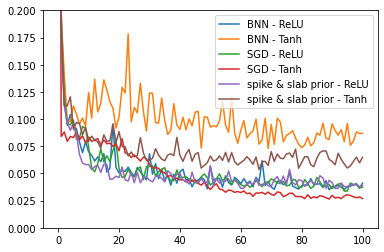
\includegraphics[width=0.45 \linewidth]{Images/Q4/c.png}}
	 \end{center}
	 \caption{{\footnotesize }}\label{Fig10}    
	\end{figure}	

		}
	\end{enumerate}
\end{enumerate}


\end{document}
